\subsection{D and B mesons}
A high statistics sample of pPb collisions will be extremely useful to test heavy-flavour production over a wide transverse momentum range.
At low $\rm p_{T}$, the study of the nuclear modification factors of D and B mesons allows to test the relevance of cold nuclear matter effects in the 
heavy flavour sector~\cite{Eskola:2009uj,deFlorian:2003qf,Frankfurt:2011cs}. Gluon saturation processes are expected to reduce the production 
cross sections of D mesons of about 10-20$\%$ at about 2-3 GeV/c.  
In the B sector, a smaller modification is expected as a consequence of the large $x_{bjorken}$ range that we can investigate.
A precise measurement of the D and B nuclear modification factor in pPb collisions at low $\rm p_{T}$ is therefore needed to experimentally validate
the theoretical expectations. In Fig~\ref{fig:Bextrapolated}, the expected statistical and systematic uncertainties on the $\rm B^{+}$ measurement 
considering an integrated luminosity of 100/nb are presented. In absence of any theoretical calculations that describe the $\rm R_{pA}$
of B the central value was set to one. In the transverse momentum region 8-10 GeV/c we would be able to measure $\rm R_{pA}$ 
of $\rm B^{+}$ with a precision better than 4-5$\%$. The high luminosity scenario is therefore needed to be able to measure B cross sections at low 
 $\rm p_{T}$ with the required accuracy.
 A larger sample of 8 TeV pPb data would also be beneficial for heavy flavour studies at high $\rm p_{T}$.  In Fig~\ref{fig:plotsDBpredictions}, 
the FONLL predictions for D (left) and B (right) cross sections are shown. A  increase of the heavy-flavour cross section of about 2 is
expected at $\rm p_{T}~$100 GeV/c as a consequence of the larger centre-of-mass value. 

\begin{figure}[h]
\begin{center}
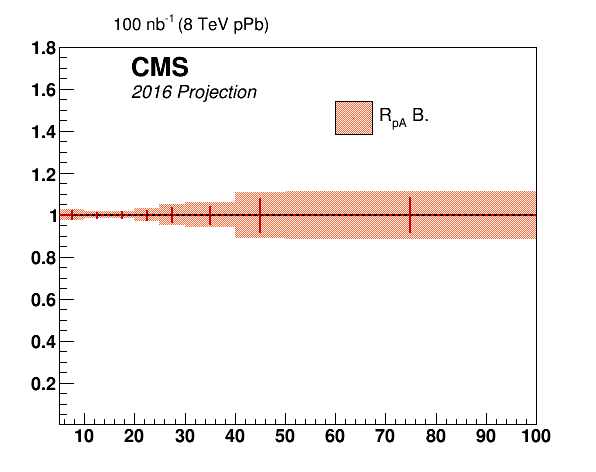
\includegraphics[width= 0.55\textwidth]{figures/BpPbprediction.jpg}
\caption{Prediction for $\rm B^{+}$ $\rm R_{pPb}$ estimated with a luminosity of $\rm L_{int}$=100/nb based on 2011 pPb measurement.}
\label{fig:Bextrapolated}
\end{center}
\end{figure}


\begin{figure}[h]
\begin{center}
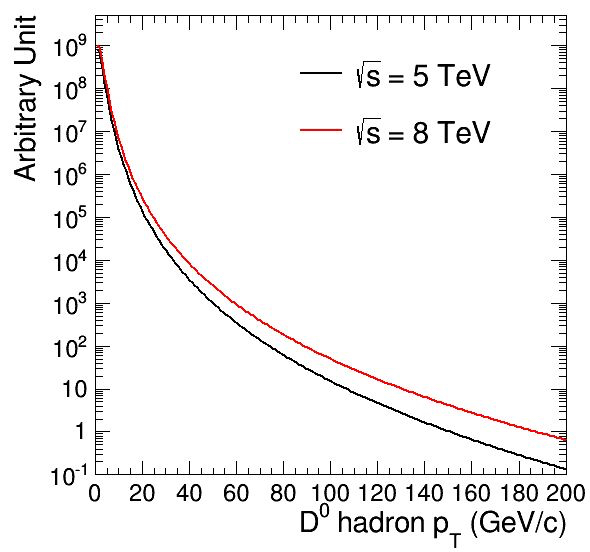
\includegraphics[width= 0.45\textwidth]{figures/D-Sigma.jpg}
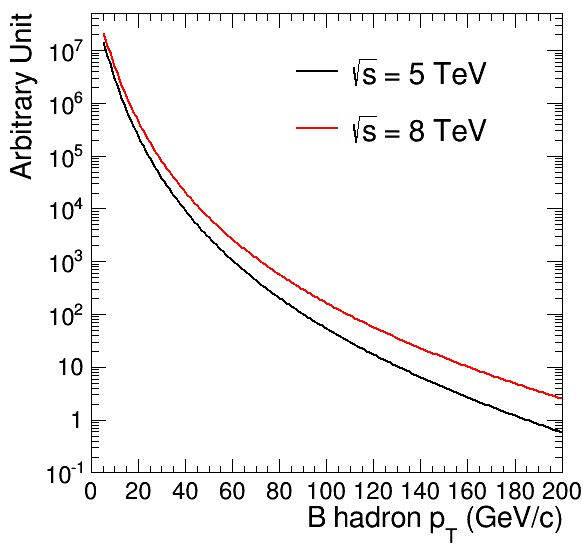
\includegraphics[width= 0.45\textwidth]{figures/B-Sigma.jpg}
\caption{FONLL predictions for D (left) and B (right) meson production at 8 and 5TeV as a function of $\rm p_{T}$~\cite{FONLLcharmbottomPP1}.}
\label{fig:plotsDBpredictions}
\end{center}
\end{figure}
